\section{Objective}
\begin{itemize}
    \item To understand the Maximum Power Transfer Theorem and determine the load resistance at which a DC source network delivers maximum power to a variable load.
    \item To experimentally plot load power against load resistance and locate the point of maximum power transfer.
    \item To compare the measured results against theoretical calculations and evaluate the percentage error.
\end{itemize}

\section{Introduction}
When a DC source network -- with some fixed internal (Thevenin) resistance -- is connected to a variable load, a natural question is what load resistance pulls the most power out of it. The \textbf{Maximum Power Transfer Theorem} answers this question directly: the load draws maximum power when its resistance is made equal to the source's own internal (Thevenin) resistance. This experiment builds a Thevenin-equivalent source circuit, sweeps a variable load resistance across a range of values, measures the load current and power at each setting, and locates the load resistance at which the power actually peaks.

\section{Theory}

\subsection{Statement of the Theorem}
A linear, two-terminal DC network delivers maximum power to a variable external load resistance $R_L$ if and only if $R_L$ is made equal to the Thevenin equivalent resistance $R_{th}$ of the network as seen from the load terminals:
\[
R_L = R_{th}.
\]

\subsection{Derivation}
If we replace the source network with its Thevenin equivalent ($V_{th}$ in series with $R_{th}$) driving a load $R_L$, the load current works out to
\[
I_L = \frac{V_{th}}{R_{th}+R_L}, \qquad P_L = I_L^2 R_L = \frac{V_{th}^2 R_L}{(R_{th}+R_L)^2}.
\]
To find the $R_L$ that maximizes $P_L$, we differentiate with respect to $R_L$ and set $\dfrac{dP_L}{dR_L}=0$, which leads to the condition $R_L = R_{th}$. At that point,
\[
I_{L(\max)} = \frac{V_{th}}{2R_{th}}, \qquad P_{L(\max)} = \frac{V_{th}^2}{4R_{th}}.
\]
It's worth noting that at this matched condition, only half of the power the source generates actually makes it to the load -- the other half is lost inside the source's own internal resistance $R_{th}$. So the \textbf{efficiency is only $50\%$} right at maximum power transfer, which shows that getting the most power out of a source and getting the most efficiency out of it are two different goals that can't both be met at once.

\section{Apparatus and Components}
\begin{table}[h!]
    \centering
    \caption{List of Equipment and Components Used}
    \vspace{2mm}
    \begin{tabular}{llc}
        \toprule
        \textbf{Item Description} & \textbf{Specification / Rating} & \textbf{Quantity} \\
        \midrule
        DC Power Supply (Thevenin source, $V_{th}$) & \qty{8}{\volt} & 1 \\
        Fixed Series Resistor $R_i$ ($=R_{th}$) & \qty{663}{\ohm} & 1 \\
        Decade Resistance Box (Variable Load $R_L$) & \qty{0}{\ohm}--\qty{5}{\kilo\ohm} & 1 \\
        Digital Multimeter (DMM) & DC Volts / DC Amps & 1 \\
        Solderless Breadboard & Standard Tie-Point & 1 \\
        Connecting Wires & Jumper Wires & As required \\
        \bottomrule
    \end{tabular}
    \label{tab:apparatus6}
\end{table}

\section{Circuit Diagram}

\begin{figure}[h!]
    \centering
    \begin{circuitikz}[american, scale=1.0]
        \draw (0,0) to[battery1, l=$V_{th}$, invert] (0,3)
              (0,3) to[R, l=$R_i$] (4,3)
              to[R, l=$R_L$, i=$I_L$] (4,0) -- (0,0);
        \draw (4,0) node[ground]{};
    \end{circuitikz}
    \caption{Thevenin-equivalent source ($V_{th}=\qty{8}{\volt}$, $R_i=\qty{663}{\ohm}$) driving a variable decade-box load $R_L$, used to trace the load-power curve.}
    \label{fig:maxpowercircuit}
\end{figure}

\section{Experimental Procedure}
\begin{enumerate}
    \item Build the Thevenin-equivalent source circuit shown in Figure~\ref{fig:maxpowercircuit}, using $V_{th}=\qty{8}{\volt}$ and an internal series resistance $R_i=\qty{663}{\ohm}$.
    \item Connect the decade resistance box across the output terminals so it acts as the variable load $R_L$.
    \item Starting from a low value, step $R_L$ up through a range of settings that go well below $R_i$ and well above it.
    \item At each setting, measure the load current $I_L$ and work out (or measure directly) the corresponding load power $P_L$.
    \item Plot $P_L$ against $R_L$, find the load resistance where the power peaks, and check it against the theoretical prediction $R_L = R_i$.
\end{enumerate}

\section{Theoretical Calculations}
With $V_{th}=\qty{8}{\volt}$ and $R_i=R_{th}=\qty{663}{\ohm}$, the theoretical load current and power at any load setting follow
\[
I_L = \frac{V_{th}}{R_{th}+R_L}, \qquad P_L = I_L^2 R_L,
\]
and the theoretical maximum power occurs exactly at $R_L=R_{th}=\qty{663}{\ohm}$:
\[
P_{L(\max)} = \frac{V_{th}^2}{4R_{th}} = \frac{8^2}{4\times663} = \frac{64}{2652} = \qty{24.13}{\milli\watt} \approx \qty{24.12}{\milli\watt}.
\]
These formulas were evaluated at each of the seven load-resistance settings used experimentally, and the results are reported alongside the measured values in Table~\ref{tab:maxpowerdata}.

\section{Data Collection}

\begin{table}[h!]
    \centering
    \caption{Experimental Measurement Log for Maximum Power Transfer Evaluation ($V_{th}=\qty{8}{\volt}$, $R_i=\qty{663}{\ohm}$)}
    \vspace{2mm}
    \resizebox{\textwidth}{!}{%
    \begin{tabular}{cccccc}
        \toprule
        \textbf{S.No.} & \textbf{$R_L$ ($\Omega$)} & \textbf{Measured $I_L$ (mA)} & \textbf{Calculated $I_L$ (mA)} & \textbf{Observed $P_L$ (mW)} & \textbf{Calculated $P_L$ (mW)} \\
        \midrule
        1 & 99.6  & 10.70 & 10.50 & 11.30 & 10.92 \\
        2 & 327   & 8.22  & 8.08  & 22.10 & 21.80 \\
        3 & 460   & 7.23  & 7.12  & 24.00 & 23.30 \\
        4 & \textbf{663 (Peak)} & \textbf{6.14} & \textbf{6.03} & \textbf{24.90} & \textbf{24.12} \\
        5 & 973   & 4.97  & 4.89  & 23.90 & 23.20 \\
        6 & 2152  & 2.88  & 2.84  & 17.80 & 17.30 \\
        7 & 3232  & 2.07  & 2.05  & 13.90 & 13.60 \\
        \bottomrule
    \end{tabular}%
    }
    \label{tab:maxpowerdata}
\end{table}

\textit{Note: Data transcribed from the instructor-reviewed handwritten laboratory data sheet (Group~04). Measured current $I_L$ was read directly with the DMM; observed power $P_L$ was computed from the corresponding measured load voltage and current.}

\begin{figure}[h!]
    \centering
    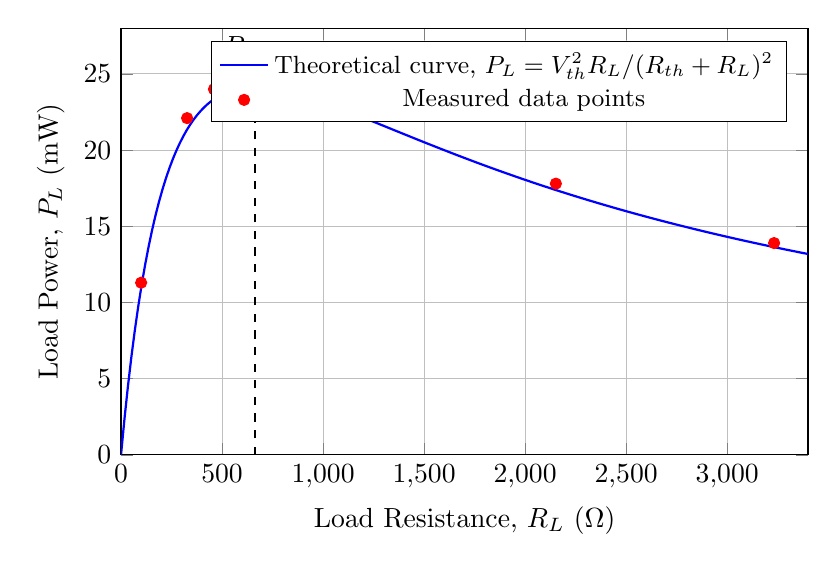
\begin{tikzpicture}
    \begin{axis}[
        width=0.85\textwidth,
        height=7cm,
        xlabel={Load Resistance, $R_L$ ($\Omega$)},
        ylabel={Load Power, $P_L$ (mW)},
        xmin=0, xmax=3400,
        ymin=0, ymax=28,
        grid=major,
        legend pos=north east,
        legend style={font=\small},
    ]
        \addplot[domain=0:3400, samples=200, thick, blue] {64000*x/(663+x)^2};
        \addlegendentry{Theoretical curve, $P_L = V_{th}^2 R_L/(R_{th}+R_L)^2$}
        \addplot[only marks, mark=*, red, mark size=2pt] coordinates {
            (99.6,11.30) (327,22.10) (460,24.00) (663,24.90) (973,23.90) (2152,17.80) (3232,13.90)
        };
        \addlegendentry{Measured data points}
        \draw[dashed] (axis cs:663,0) -- (axis cs:663,24.90);
        \node[above] at (axis cs:663,25.3) {$P_{max}$};
    \end{axis}
    \end{tikzpicture}
    \caption{Load power $P_L$ versus load resistance $R_L$, plotted from the measured data of Table~\ref{tab:maxpowerdata}. The peak occurs at $R_L \approx \qty{663}{\ohm} = R_i$, consistent with the Maximum Power Transfer Theorem.}
    \label{fig:maxpowergraph}
\end{figure}

\section{Result Analysis}
Looking at Table~\ref{tab:maxpowerdata}, the observed load power hits its highest value right at $R_L=\qty{663}{\ohm}$ ($P_{L}=\qty{24.90}{\milli\watt}$), which is exactly the internal resistance $R_i$ -- just what theory predicts. Comparing this peak to the theoretical maximum,
\[
\text{\% Error} = \left|\frac{P_{L(\max,\text{calc})}-P_{L(\max,\text{obs})}}{P_{L(\max,\text{calc})}}\right|\times100\% = \left|\frac{24.12-24.90}{24.12}\right|\times100\% \approx 3.23\%.
\]
As Figure~\ref{fig:maxpowergraph} shows, the power curve rises on both sides of $R_L=\qty{663}{\ohm}$ and there's only one peak, right where it should be, which confirms the Maximum Power Transfer Theorem.

\section{Discussion and Sources of Error}
The percentage error at the peak was about $3.23\%$, so overall the results back up the theory reasonably well. Still, a few things in the real setup keep it from matching the ideal calculations exactly:
\begin{enumerate}
    \item \textbf{Resistor Tolerance:} $R_i$ is not exactly its labeled value -- every resistor is only guaranteed to within a manufacturer tolerance -- so there's already a small gap between what the theory assumes and what's actually in the circuit.
    \item \textbf{Power Supply Regulation:} The DC supply output can shift slightly once it's under load, which adds a bit of error at each load setting.
    \item \textbf{Multimeter Loading:} An ammeter isn't a true zero-resistance short -- it has some small burden resistance -- and a voltmeter isn't a true infinite resistance either, so just connecting the meters changes the circuit slightly from what's assumed in the calculations.
    \item \textbf{Decade Box and Contact Resistance:} The decade box can only be set in discrete steps, and the breadboard and jumper wires add a bit of contact resistance that the ideal model doesn't account for. This shows up most clearly near the peak of the power curve, where $R_L$ is close to $R_i$ and the curve is changing shape quickly.
\end{enumerate}

\section{Conclusion}
This experiment confirmed the Maximum Power Transfer Theorem for a DC network. The load power measured across seven $R_L$ settings traced out the expected curve, peaking right at $R_L=\qty{663}{\ohm}$, which matches the source's internal resistance $R_i$ almost exactly, with a percentage error of only about $3.23\%$ at the peak. That confirms the matching condition $R_L=R_{th}$ predicted by theory, and it also illustrates the trade-off between power and efficiency mentioned earlier -- getting the most power out of the source means running at only 50\% efficiency, since half of the power is used up inside the source itself.

\section{References}
\begin{tcolorbox}[colback=gray!5, colframe=gray!40, arc=2mm]
\begin{enumerate}
    \item Alexander, C. K., \& Sadiku, M. N. O. (2016). \textit{Fundamentals of Electric Circuits} (6th ed.). McGraw-Hill Education. (Chapter 4: Circuit Theorems).
    \item Hayt, W. H., Kemmerly, J. E., \& Durbin, S. M. (2012). \textit{Engineering Circuit Analysis} (8th ed.). McGraw-Hill Education. (Chapter 5: Useful Circuit Analysis Techniques).
    \item Boylestad, R. L. (2015). \textit{Introductory Circuit Analysis} (13th ed.). Pearson. (Chapter 9: Network Theorems).
\end{enumerate}
\end{tcolorbox}

\clearpage
\section{Appendix: Signed Data Sheet}
\begin{figure}[h!]
    \centering
    \includegraphics[width=0.75\textwidth, keepaspectratio]{datasheet/exp6_datasheet}
    \caption{Instructor-signed laboratory data sheet for this experiment.}
    \label{fig:datasheet6}
\end{figure}
